
\subsubsection{17.11.14}

\begin{enumerate} 
	\item The time of beginning and ending of the meeting:
	18:00 - 20:40
	\item Purposes of the meeting:
	\begin{enumerate}
		\item To improve the construction of bucket.
		
		\item To test the working of bucket.
		
	\end{enumerate}
	
	\item Work, that has been done:
	\begin{enumerate}
		\item Bucket was improved:
		\begin{enumerate}
			\item Inside the tube was placed plastic bottle. Tube was extended by another one bottle for more accuracy of throwing the balls into the basket.
			
			\item They were fixed plastic stripes at the bottom part of bucket. They will help to balls to enter the pipe and not get stuck.
			
			\item The bottom of bucket was bended as a boat. It allowed to balls doesn't fall outside the bucket during the raise of it.
			
			\item It was left only hole at center of bucket for hit the balls inside. It also allows to reduce risk of falling balls outside the bucket during the rise.
			
		\end{enumerate}
		
	    \begin{figure}[H]
			\begin{minipage}[h]{0.47\linewidth}
				\center{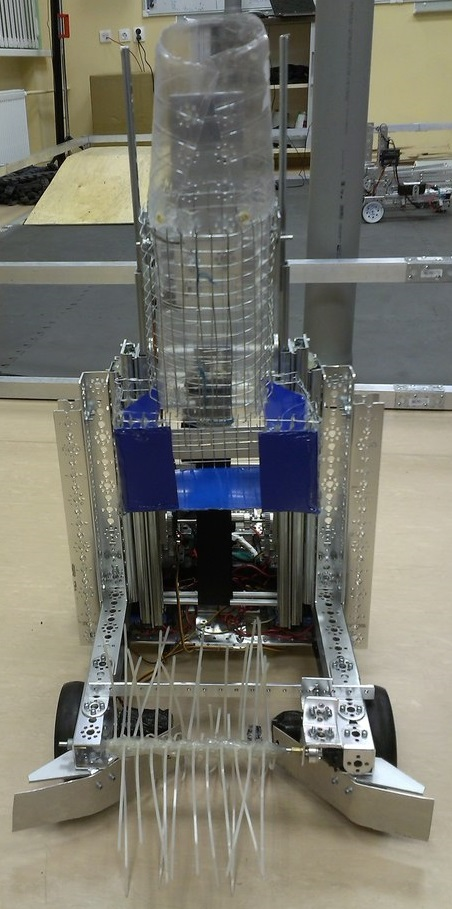
\includegraphics[scale=0.3]{days/17.11.14/images/01}}
				\caption{Bucket in vertical position}
			\end{minipage}
			\hfill
			\begin{minipage}[h]{0.47\linewidth}
				\center{
\includegraphics[scale=0.3]{days/17.11.14/images/02}}
				\caption{Bucket in overturned position}
			\end{minipage}
		\end{figure}
		
		
		\item The bucket was tested manually. Bucket can fill 2 big and 3 small balls. It is enough because at every big ball there is 3 small. Balls doesn't fall outside the bucket during the rise.
		
		
	\end{enumerate}
	
	\item Results:
	\begin{enumerate}
		\item Construction of the bucket was finished.
		
		\item Problems weren't detected during the tests of bucket.
		
	\end{enumerate}
	
	\item Tasks for the next meetings:
	\begin{enumerate}
		\item To test the bucket with help programme.
		
	\end{enumerate}     
\end{enumerate}
\fillpage

